\documentclass[a4paper]{article}

%--------------------------------------------------------------------------
\usepackage[a4paper, total={6in, 9in}]{geometry}
\usepackage{amsmath}
\usepackage{booktabs}
\usepackage{caption}
\usepackage{graphicx}
\usepackage{float}
\usepackage{inconsolata}
\usepackage{listings}
\usepackage{xcolor}
\usepackage{siunitx}
\usepackage[most]{tcolorbox}
\usepackage{etoolbox}

\makeatletter
\patchcmd{\l@section}
{\hfil}
{\leaders\hbox{\normalfont$\m@th\mkern \@dotsep mu\hbox{.}\mkern \@dotsep mu$}\hfill}
{}{}
\makeatother

%--------------------------------------------------------------------------
\graphicspath{{./fig/}}

%--------------------------------------------------------------------------

\definecolor{mGreen}{rgb}{0,0.6,0}
\definecolor{mGray}{rgb}{0.5,0.5,0.5}
\definecolor{mPurple}{rgb}{0.58,0,0.82}
\definecolor{backgroundColour}{rgb}{0.95,0.95,0.92}

\lstdefinestyle{CStyle}{
	backgroundcolor=\color{backgroundColour},   
	commentstyle=\color{mGreen},
	keywordstyle=\color{magenta},
	numberstyle=\tiny\color{mGray},
	stringstyle=\color{mPurple},
	basicstyle=\footnotesize,
	breakatwhitespace=false,         
	breaklines=true,                 
	captionpos=b,                    
	keepspaces=true,                 
	numbers=left,                    
	numbersep=5pt,                  
	showspaces=false,                
	showstringspaces=false,
	showtabs=false,                  
	tabsize=2,
	language=C
}

\setlength\parindent{0pt}

%--------------------------------------------------------------------------
\begin{document}
\title{HIT332: Embedded and Mobile Systems\\ Practical 3 Notes}
\author{Shane Reynolds}
\maketitle

\tableofcontents

%--------------------------------------------------------------------------
\section{Introduction \& Background}
The intention behind this brief set of notes is to provide guidance on how well the practicals and projects for HIT332: Embedded and Mobile Systems achieve their intended outcomes. There are 5 practicals in total, and 3 projects. This set of notes will cover Practical 3. The practicals (and projects) make use of a development board created by Damien Hill and Ben Saunders of Charles Darwin University. The main component of the board is the Atmel ATmega1281 16au 16MHz, 8-bit microcontroller. The development board can be seen in Figure 1.

\begin{figure}[h]
	\centering
	\frame{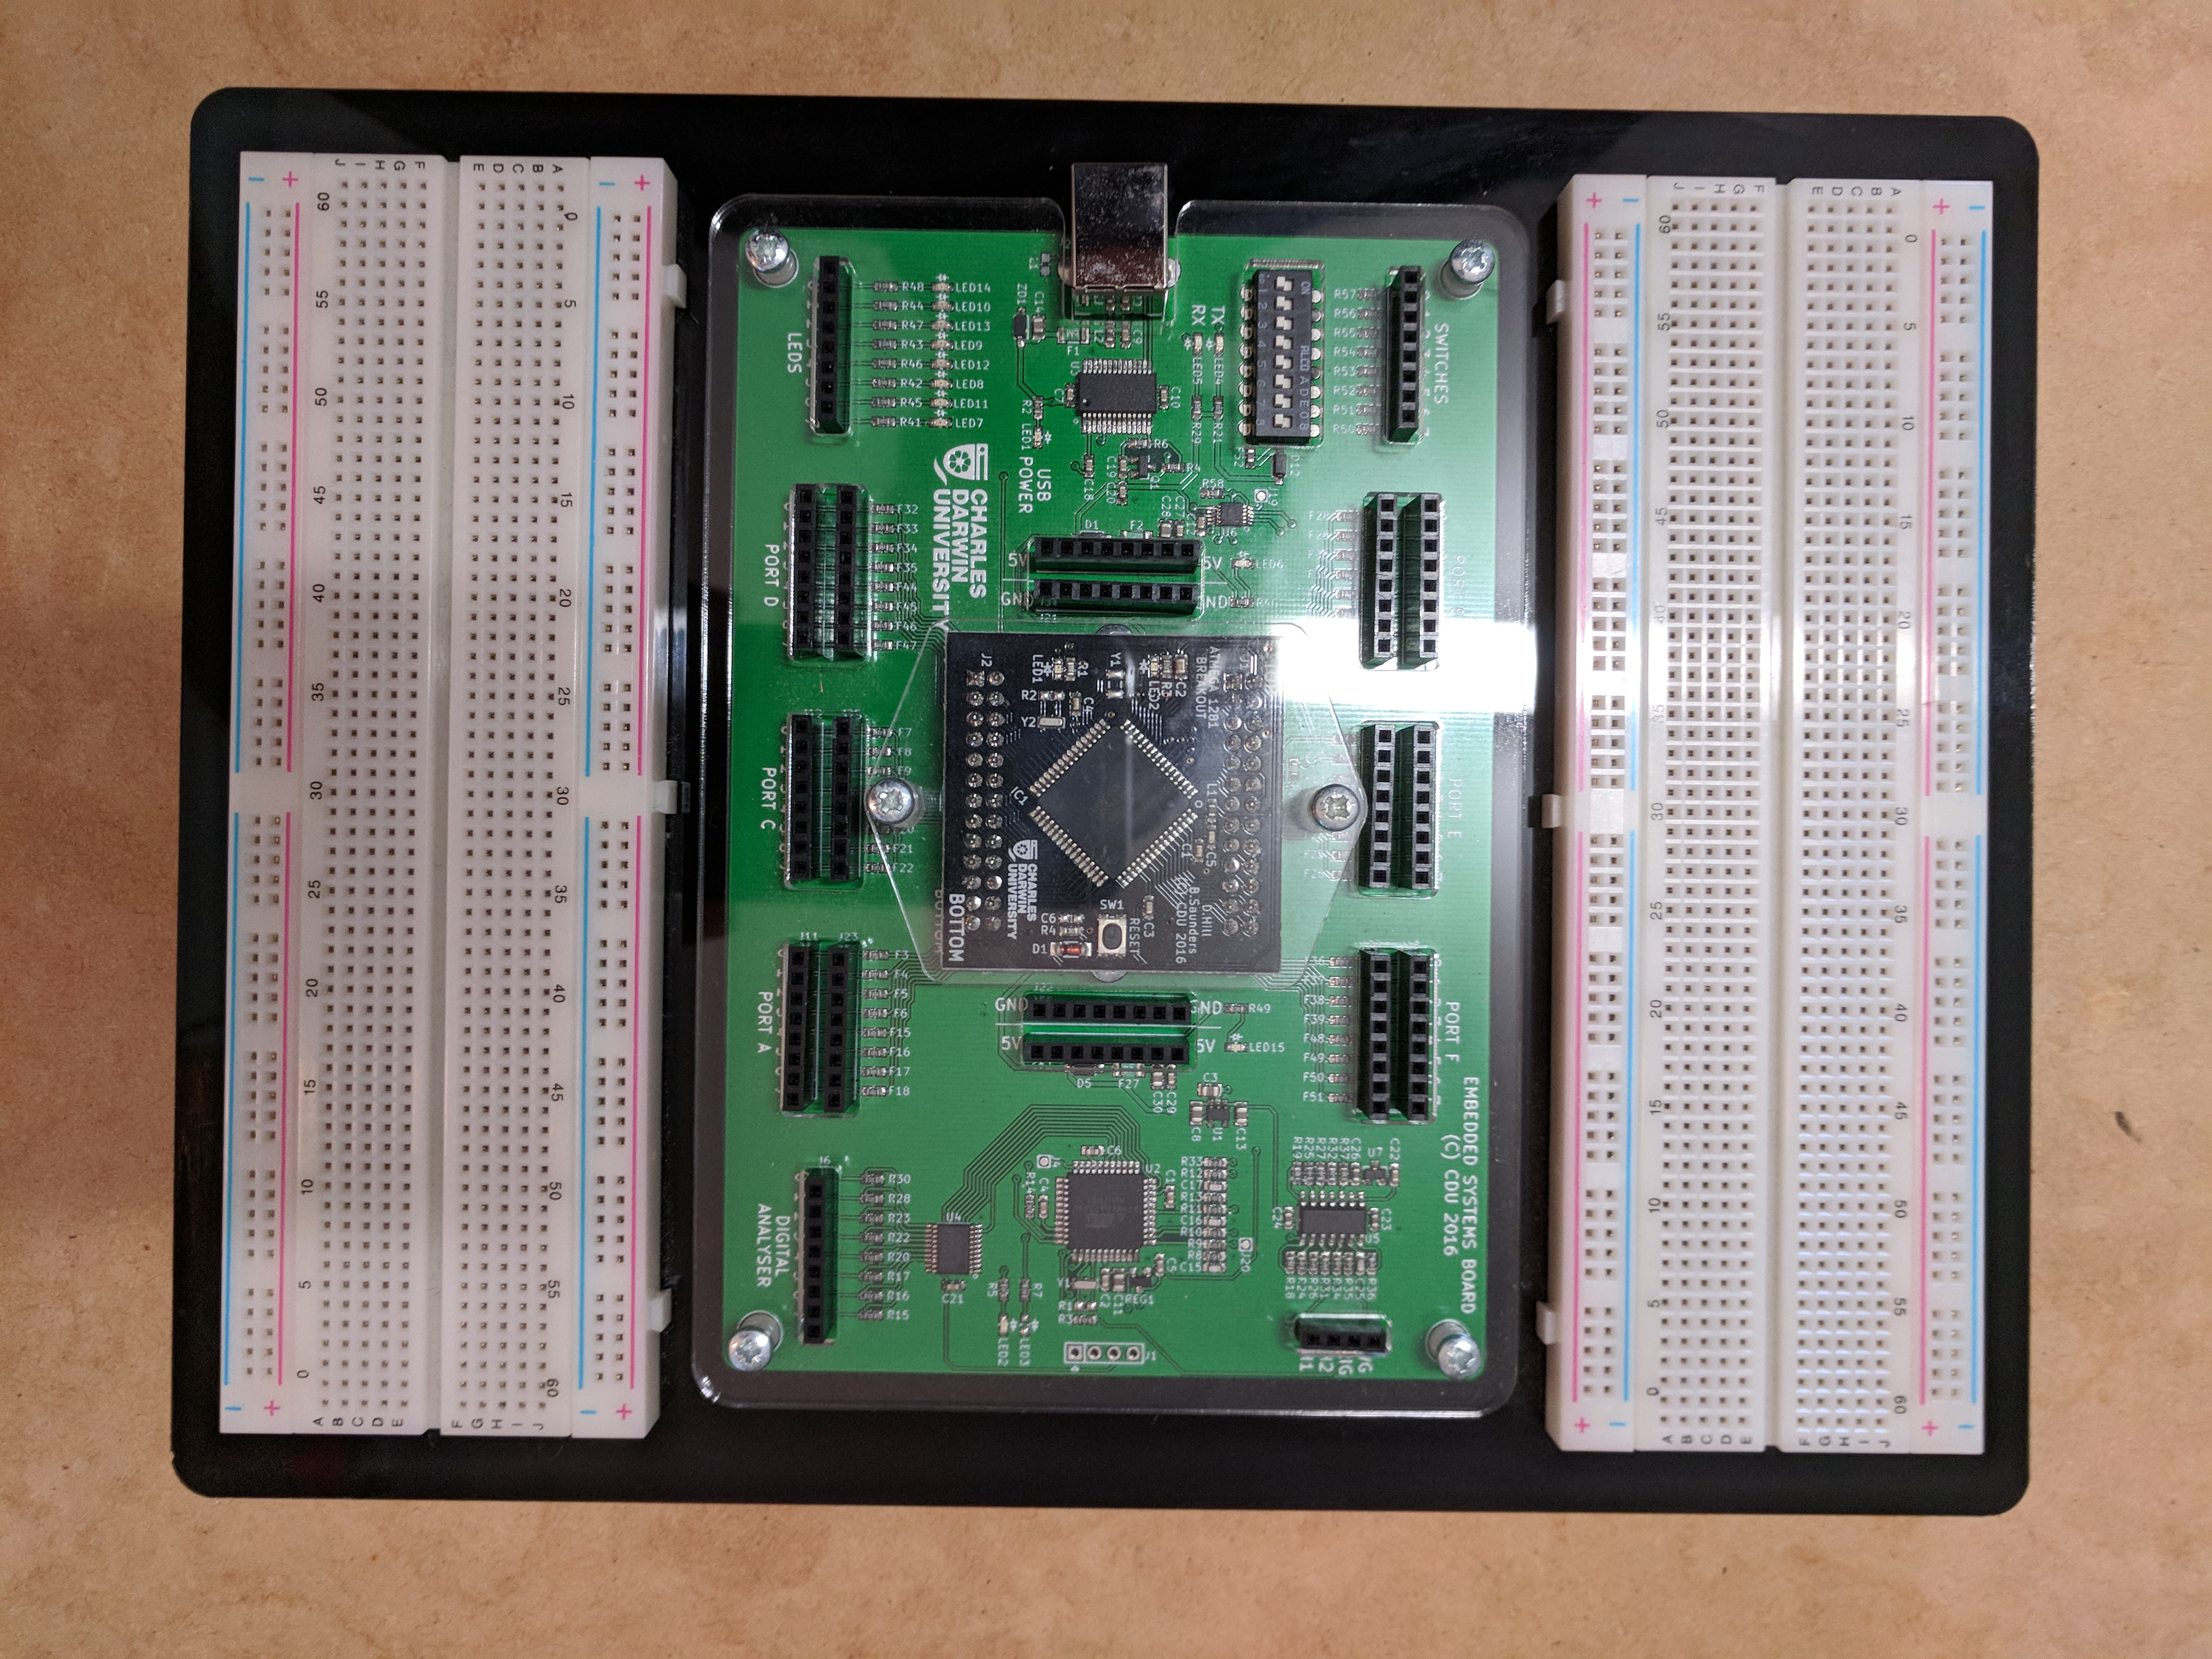
\includegraphics[scale=0.05]{fig1}}
	\caption{The development board which is used in practicals and projects for HIT332: Embedded and Mobile Systems}
\end{figure}

It must be highlighted that these notes have been developed using the board outside of its intended ecosystem. The board is made to be used on CDU's Casuarina Campus in one of the Engineering computer labs. These labs have the appropriate software installed in the correct file paths. These notes have been written using software installed on a personal machine which CDU does not control. Furthermore, the components (other than the development board) used to complete the exercises were sourced independently from a local electronics supplier, independently of CDU. The notes will be highlighted where there has been a significant departure from the intended experience.

\section{Digital Input and Output}

\begin{figure}[h]
	\begin{lstlisting}[style=CStyle]
	/*#include <avr/io.h>*/
	#include <avr/io.h>
	
	int main (void){
		/*This configuration has Port B as an input port, and a high is placed on each pin using software. Furthermore, we have Port D configured as an output port - we note that a logical zero is set up to be interpreted as a voltage HIGH (i.e. 0 = ON and 1 = OFF). Finally there is a piece of software that sets PORTD equal to PINB - I'm not quite sure how PINB works though*/
	
		/*The dip switches are attached to PORT B, and the LED attached to Port D. When initially connected the dip switches are all off, which means that the software 1 is passed to Port B and the LED are turned off. When a dip switch is turned on, then we get 1 + 1 (??) at the specific pin at Port B, which then reigsters as a 0 and is passed to Port D which turns on the LED*/
	
		/*If one of the dip switches is disconnected from port B then the corresponding LED switches on. What is happening here?*/
	
		DDRB = 0x00; /*DDRB written logic 0 - configured as input*/
		PORTB = 0x00; /*PORTB has the input 1111 1111 placing a software HIGH on each pin.
		I'm not actually sure what this second line does...*/
	
		DDRD = 0xFF; /*DDRD has a written logic 1 - configured as output*/
		PORTD = 0x00; /*PORTD is output and written logic 0 - configured as driven low*/
	
		while(1){
			PORTD = PINB;
		}
	}
	\end{lstlisting}
	\caption{text}
\end{figure}

\begin{enumerate}
	\item \textbf{Study the C code and explain the operation.}\\ Answer here
	\item \textbf{How would you expect the processor to behave if the pins on PORTB were driven high or low by an external circuit?}\\ Answer here
	\item \textbf{What would the result be if LEDs were connected to the pins on PORTD?}\\ Answer here
	\item \textbf{What happens if the pins on PORTB are left unconnected (floating)?}\\ Answer here
\end{enumerate}
\section{Using Make and Makefiles}

\section{KiCAD Schematic}

\section{Wiring the Board and Programming Embedded Program}



\end{document}